\documentclass[crop,border=5pt,convert]{standalone}

\usepackage{tikz,comment}
\usetikzlibrary{calc,backgrounds}

\usepackage{pgfplots}
\pgfplotsset{compat=1.11}

\tikzset{background fill/.style={background rectangle/.style={fill=#1},show background rectangle}}



\begin{document}
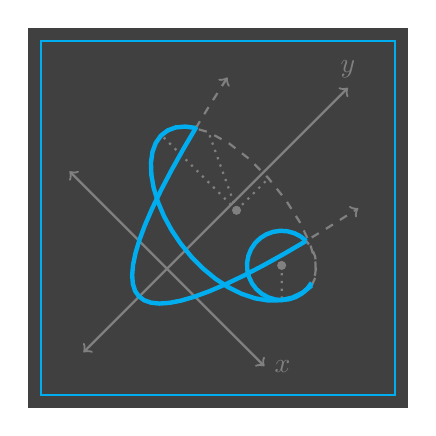
\begin{tikzpicture}[background rectangle/.style={fill=darkgray}, show background rectangle]
\draw (-1.25,-1.25) rectangle (3.25,3.25) [cyan,thick];
% draw axes
\draw[<->,thick,gray,rotate=-45] (-1.75,.5) -- (1.75,.5) node[right]{$x$};
\draw[<->,thick,gray,rotate=-45] (0,-1) -- (0,3.75) node[above]{$y$};
% draw x^2
\def\a{1};
\def\b{2};
\draw[<->,thick,gray,dashed,domain=-\a-.175:\a+.175,rotate=-45] plot ({\x},{(\b/(\a^2))*(\x)^2});
% draw ellipse
\draw[thick,gray,dashed,domain=0:360,rotate=-45] plot ({1.35*cos(\x)+.1},{(.2*\x/145+.45)*sin(\x)+1.65});
% draw ellipse guides
\draw[rotate=-45,fill=gray,gray] (.1,1.65) circle (.05cm);
\draw[rotate=-45,gray,dotted,thick] (.1,1.65) -- ({1.35*cos(180)+.1},{(.2*180/145+.45)*sin(180)+1.65});
\draw[rotate=-45,gray,dotted,thick] (.1,1.65) -- ({1.35*cos(90)+.1},{(.2*90/145+.45)*sin(90)+1.65});
\draw[rotate=-45,gray,dotted,thick] (.1,1.65) -- ({1.35*cos(90+45)+.1},{(.2*(90+45)/145+.45)*sin(90+45)+1.65});
% draw circle
\draw[thick,gray,dashed,domain=0:360,rotate=-45] plot ({\b*\a*1.1*cos(\x)/(5)+\a},{\b*\a*1.1*sin(\x)/(5)+\b-\b*\a*1.1/(5)});
% draw circle guides
\draw[rotate=-45,fill=gray,gray] (\a,\b-\b*\a*1.1/5) circle (.05cm);
\draw[rotate=-45,gray,dotted,thick] (\a,\b-\b*\a*1.1/5) -- ({\b*\a*1.1*cos(-45)*(1/5)+\a},{\b*\a*1.1*sin(-45)/5+\b-\b*\a*1.1/5});
% draw &e (Andy)
\draw[ultra thick,cyan,domain=145:360,rotate=-45] plot ({1.35*cos(\x)+.1},{(.2*\x/145+.45)*sin(\x)+1.65});
\draw[ultra thick,cyan,domain=90:375,rotate=-45] plot ({\b*\a*1.1*cos(\x)/(5)+\a},{\b*\a*1.1*sin(\x)/(5)+\b-\b*\a*1.1/(5)});
\draw[ultra thick,cyan,domain=-\a-.01:\a,rotate=-45] plot ({\x},{(\b/(\a^2))*(\x)^2});
\end{tikzpicture}

\end{document}
